\chapter{GAN}
Ein \glqq Generative Adversarial Net\grqq{} besteht aus zwei Teilstücken. Der erste Teil wird \glqq generative model $G$\grqq{}
genannt und generiert auf Basis eines originalen Datensets neue Datensamples. Der zweite Teil nennt sich \glqq discriminative model $D$\grqq{}
und schätzt die Wahrscheinlichkeit, ob ein solches Sample, welches $G$ generiert, aus dem originalen Datenset stammt. $D$
selbst hat als Output also eine reele Zahl. \cite{8253599}
In den Worten der Autoren ausgedrückt ist ein \Gls{GAN} ein Spiel zwischen Geldfälschern und Polizisten:
\itenquote{The generative model can be thought of as analogous to a team of counterfeiters,
trying to produce fake currency and use it without detection, while the discriminative model is
analogous to the police, trying to detect the counterfeit currency. Competition in this game drives
both teams to improve their methods until the counterfeits are indistiguishable from the genuine
articles} \cite{8253599}.
Anders ausgedrückt versucht $G$ immer besser zu werden, um $D$ möglichst zu überlisten. $D$ hingegen sieht sich einem immer
besser werdenden $G$ gegenüber gestellt und muss seine eigenen Schwachstellen ausbessern, um $G$ entgegenzuhalten. Eine Architektur, die
so aufgebaut ist, dass sie sich gegenseitig immer weiter verbessert. Aus diesm Grund auch \glqq Generative \textbf{Adversarial} Net\grqq{} genannt.
\para
Im Endeffekt besteht das Ziel also darin, dass $D$ nicht mehr sagen kann, ob ein Sample von $G$ oder aus dem originalen Datenset stammt.
Somit sollte $D$ für alle Samples immer $\frac{1}{2}$ ausgeben. Dies bedeutet, dass ein Sample dieselbe Wahrscheinlichkeit
hat aus dem originalen Datenset oder aus dem generierten Set zu stammen und diese
beiden Datensets daher nicht mehr unterscheidbar sind.
Der Trainingsprozess für $G$ kann weiterhin als Maximierung der Fehlerwahrscheinlichkeit für $D$ angegeben werden. Dies entspricht also einem
Zwei-Spieler Minimax-Algorithmus, auf welchen in dieser Arbeit ebenfalls noch eingegangen wird.\cite{8253599}
\para
Das generative Modell $G$ sowie das unterscheidende Modell $D$ bestehen jeweils aus zwei \Glspl{Multilayer perceptron}. Dies hat
den Vorteil, dass die Modelle mittels \Gls{Backpropagation} trainiert werden können \cite{8253599}.

\section{Neuronale Netze - Multilayer Perceptron}
Da die Architektur des \Gls{GAN} auf zwei neuronalen Netzen beruht, wird in diesem Kapitel kurz darauf eingegangen. Dieser
Einschub gibt einen groben Überblick, hat aber nicht die Absicht, ein vertieftes Wissen zu vermitteln.
\para
Die neuronalen Netze sind, wie so manches, über die Zeit herangereift. Die Intention besteht nicht darin, das menschliche Gehirn
nachzubauen, sondern eher eine Art Modell für die Informationsverarbeitung zu beschreiben \cite{wiki:knn}. Wie in der Biologie versucht man dies
in diesen Netzen über Neuronen, wo auch der Name herrührt. Ein solches
Neuron bekommt als Eingabe eine Summe von gewichteten Werten, welche es durch eine sogenannte \glqq Aktivierungsfunktion\grqq{} in
einen Ausgabewert umwandelt.
\para
Am Anfang dieser Netzwerke stand das Perzeptron, welches nur ein
einziges künstliches Neuron beinhaltet und von Frank Rosenblatt beschrieben wurde.\cite{wiki:perzeptron} Danach hat man damit
begonnen, diese Neuronen über Layer miteinander zu verbinden, wobei man den ersten Layer als Input-Layer, die Layer dazwischen
als Hidden-Layer und den letzten Layer aus Output-Layer kennt. Der Output-Layer beinhaltet in einem einfachen \Gls{KNN} so viele
Neuronen, wie es Klassen gibt. Jedes dieser Output-Neuronen gibt die Wahrscheinlichkeit an, ob eine Eingabe zu der jeweiligen
Klasse gehört \cite{wiki:knn}.
\para
Ein solches neuronales Netz ist eigentlich eine Optimierungsaufgabe. In dem Fall geht es darum, am Ende eine Fehlerfunktion, welche
den Abstand des Ist- und Sollzustands beschreibt, zu minimieren. Je geringer der Fehler, desto besser klassifiziert das Netz. Die
Variablen, welche dabei angepasst werden können, sind die Gewichte, welche jeweils auf einer Verbindung zwischen zwei Neuronen liegen.
Wie wahrscheinlich jeder aufmerksame Leser erkennt, werden dies sehr schnell sehr viele Variablen, weswegen normale Verfahren wie
z.B. der Gradientenabstieg zwar eingesetzt werden können, aber sehr ineffizient sind.
Der Durchbruch dieser Netzwerke wurde daher erst mit der Beschreibung des \Gls{Backpropagation}-Algorithmus erzielt, welcher ein Spezialfall
des Gradientenabstiegverfahrens darstellt und die Gewichte aufgrund ihres Anteils am Fehler anpasst \cite{wiki:backpropagation}.
Heute gibt es sehr viele verschieden Arten und Architekturen von künstlichen neuronalen Netzen, auf welche nun nicht weiter eingegangen
wird.

\section{Funktionsweise}
Formell ausgedrückt besteht ein \Gls{GAN} aus zwei ableitbaren Funktionen $G(z;\theta_g)$ und $D(x,\theta_d)$, welche durch zwei \Glspl{Multilayer perceptron}
dargestellt werden. Dabei bilden jeweils $\theta_g$ sowie $\theta_d$ die Parameter der Netzwerke. Um die generierten Daten $p_g$ über ein Sample $x$ aus
dem originalen Datenset $p_{data}$ zu trainieren, wird eine Input-Noise-Funktion $p_z(z)$ definiert. $G(z;\theta_g)$ bildet dabei das
Mapping zwischen diesen Noise-Daten und dem originalen Datenset $p_{data}$.
Aus dem Noise wird also ein Sample erzeugt, welches möglichst mit den Samples aus $p_{data}$ korreliert.
$D(x)$ wiederum gibt einen einzelnen Skalar aus, der die Wahrscheinlichkeit beschreibt, ob ein Sample $x$ eher aus dem originalen Datenset $p_{data}$
als aus dem generierten Datenset $p_g$ (beinhaltet alle Samples von $G$) stammt.
$D$ wird nun so trainiert, um die Wahrscheinlichkeit zu maximieren, das korrekte Label einem Input-Sample $x$ zu geben. Dabei gibt es zwei Labels:
\glqq Stammt aus original Datenset\grqq{} und \glqq Stammt aus generiertem Datenset\grqq{}. Simultan dazu wird $G$ trainiert, um die Funktion
$\log(1 - D(G(z)))$ zu minimieren\cite[p.~1]{8253599}. In Worten: $G(z)$ generiert ein Sample aus den Noise-Daten.
Davon wird die Wahrscheinlichkeit berechnet, ob dieses Sample aus dem originalen Datenset stammt. Wird dieser Wert gross, das heisst,
$D$ hat das Gefühl, dass das generierte Sample aus dem originalen Datenset stammt, so geht der Wert innerhalb des Logarithmus gegen 0 und damit gegen $-\infty$.
Dadurch wird also über diese Minimierung erzielt, dass $G$ möglichst Daten generiert, die $D$ nicht dem generierten Datenset sondern dem originalen Datenset selbst zuweist.
Die Autoren verweisen hier auf die Tatsache, dass die beiden neuronalen Netze $D$ und $G$ ein
Zwei-Spieler minimax-Spiel mit der folgenden Value-Funktion $V(G,D)$ spielen \cite[p.~2]{8253599}:
\begin{align}
    \min_{G} \max_{D} V(D, G) = E_{x\sim p_{data}(x)}[\log D(x)] + E_{z\sim p_z(z)}[\log(1 - D(G(z)))] \label{eq:1}
\end{align}
Nachfolgend werden einige Gedanken des Autors dazu aufgeführt.\\
\textbf{Fall 1 - Discriminator macht alles richtig}:
\begin{align}
    D(x) = 1, D(G(z)) = 0 \Rightarrow \log(1) + \log(1 - 0) = \log(1) + \log(1) = 0
\end{align}
\textbf{Fall 2 - Discriminator kann nicht mehr unterscheiden}:\\
\begin{align}
    D(x) = \frac{1}{2}, D(G(z)) = \frac{1}{2} \Rightarrow \log(\frac{1}{2}) + \log(1 - \frac{1}{2}) = \log(\frac{1}{2}) + \log(\frac{1}{2}) = -\log(4) = -1.3862
\end{align}
Nach den Autoren bildet der Fall 2 das globale Minimum, welches eben nur erzielt werden kann, wenn der Discriminator nicht mehr zwischen
den beiden Datensets unterscheiden kann \cite[p.~4-5]{8253599}. Es gilt: $p_{data} = p_{g}$
Was genau diese sogenannte Value-Funktion $V(G,D)$ darstellt und wie sie hergeleitet wurde, wird im nächsten Abschnitt
genauer erläutert.
\para
Nun stellt sich also noch die Frage, wie denn genau $G$ lernt. Nach \glqq Computerphile\grqq{} erhält $G$ Informationen von $D$.
$G$ kennt also die Schwächen von $D$ und kann diese besser ausnützen \cite{youtube:gan}. Um dies besser zu verstehen,
wurde ein Artikel hinzugezogen, welcher sich einem Beispiel in Tensorflow widmet \cite{tensorflow:1:gan}. Dort
wird eine Loss-Funktion\footnote{Die Loss-Function bildet die Bewertung eines neuronalen Netzes. Sie gleicht eine Menge von Wahrscheinlichkeiten eines
Ereignisses mit einer anderen ab und soll $0$ ergeben, wenn die Mengen identisch sind.\cite{wiki:lossFunction}}
sowohl für den Generator, wie auch den Discriminator angegeben. Die Loss-Funktionen werden im nachfolgenden einzeln besprochen. Zuerst wird sich dem Generator gewidmet.
\begin{lstlisting}
    def generator_loss(fake_output):
        return cross_entropy(tf.ones_like(fake_output), fake_output)
\end{lstlisting}
Die Loss-Funktion nach \cite{tensorflow:1:gan} für den Generator besteht also im Wesentlichen aus einer Kreuzentropie\footnote{Beschreibung in
Anhang \ref{anhang:kreuzentropie}} zwischen der Wahrscheinlichkeit des Diskriminators für die generierten Samples
sowie der Wahrheit (alle Wahrscheinlichkeiten sind in dem Fall $1$). Dies bedeutet, der Fehler für den Generator ist $0$, wenn der Diskriminator
alle generierten Samples als Sample aus dem originalen Datenset anerkennt.\\
Für den Diskriminator ist die Sache ein wenig komplizierter \cite{tensorflow:1:gan}.
\begin{lstlisting}
    def discriminator_loss(real_output, fake_output):
        real_loss = cross_entropy(tf.ones_like(real_output), real_output)
        fake_loss = cross_entropy(tf.zeros_like(fake_output), fake_output)
        total_loss = real_loss + fake_loss
        return total_loss
\end{lstlisting}
An dieser Stelle werden nun die einzelnen Zeilen der Gleichung \ref{eq:1} zugewiesen. Dazu muss bekannt sein, dass der
Diskriminator ein binäres Problem beschreibt. Weiterhin scheint die Gleichung \ref{eq:1} der Kreuzentropie entnommen zu sein. Diese
kann für einen binären Klassifizierer wie in Formel \ref{eq:7} geschrieben werden \cite{stackoverflow:1:crossEntropy}.
\begin{align}
    H(P,Q) = - \sum_{x \in X} (P(x) \cdot log(Q(x)) + (1 - P(x)) \cdot log(1 - Q(x))) \label{eq:7}
\end{align}
Die erste Zeile der \glqq discriminator\textunderscore loss\grqq{} Funktion berechnet die Kreuzentropie zwischen den Wahrscheinlichkeiten der originalen Samples
sowie der erwarteten Wahrscheinlichkeiten von $D$ für die originalen Samples. Für den Diskriminator entspricht $P(x) = 1$ für alle Wahrscheinlichkeiten,
wobei $Q(x) = D(x)$ gilt und das Sample $x$ aus $p_{data}$ stammt. Eingesetzt in Formel \ref{eq:7} ergibt dies \ref{eq:8}.
\begin{align}
    H(P,Q) = - \sum_{x \in p_{data}} (P(x) \cdot log(D(x)) + (1 - P(x)) \cdot log(1 - D(x))) \label{eq:8}\\
    H(P,Q) = - \sum_{x \in p_{data}} log(D(x)) \label{eq:11}
\end{align}
Die darauffolgende Zeile der Funktion \glqq discriminator\textunderscore loss\grqq{} wird dem zweiten Summand der Gleichung \ref{eq:1} zugewiesen.
In diesem Fall ist $P(x) = 0$ für alle erwarteten Wahrscheinlichkeiten (das generierte Sample gehört nicht zum
originalen Datenset), $Q(x) = D(x)$ und $x$ stammt aus $p_{g}$.
\begin{align}
    H(P,Q) = - \sum_{x \in p_{g}} (P(x) \cdot log(D(x)) + (1 - P(x)) \cdot log(1 - D(x)))\\
    H(P,Q) = - \sum_{x \in p_{g}} log(1 - D(x)) \label{eq:9}
\end{align}
Wenn nun in Betracht gezogen wird, dass $x$ nicht aus $p_g$ stammt, sondern aus den Noise-Samples $p_z$ und $x = z$ gilt,
dann kann die Formel \ref{eq:9} so umgeschrieben werden, dass sie mit der Formel \ref{eq:1} korreliert.
\begin{align}
    x(z) = G(z)\\
    H(P,Q) = - \sum_{z \in p_{z}} log(1 - D(G(z))) \label{eq:10}
\end{align}
Zusammenaddiert ergeben die Formeln \ref{eq:11} und \ref{eq:10} fast den Loss-Wert der Formel \ref{eq:1} und damit auch die Minimax-Value-Funktion,
welche nach den Formeln \ref{eq:11} und \ref{eq:10} eigentlich von $D$ minimiert werden will.
\begin{align}
    \widetilde{V(D,G)} = - \sum_{x \in p_{data}} log(D(x)) - \sum_{z \in p_{z}} log(1 - D(G(z)))
\end{align}
$-1$ soll nun noch ausgeklammert werden, damit wird ersichtlicht, dass es sich allem Anschein nach um die
umgedrehte Loss-Function von $D$ handelt.
\begin{align}
    \widetilde{V(D,G)} = - (\sum_{x \in p_{data}} log(D(x)) + \sum_{z \in p_{z}} log(1 - D(G(z))))\\
    \widetilde{V(D,G)} = - V(D,G)\label{eq:12}
\end{align}
Formel \ref{eq:12} erklärt nun den Zusammenhang zwischen der Loss- wie auch der Value-Function aus Formel \ref{eq:1}.
Für den Minimax-Algorithmus wird also die Richtung der Optimierung umgedreht, um nach $G$ zu minimieren.

\newpage
\subsection{Einschub - Minimax}
Um zu verstehen, wieso es sich hierbei um einen solchen Minimax-Algorithmus handelt, wird in diesem Abschnitt ebendieser mit
Verweis auf die Gleichung \ref{eq:1} eingeführt. Der Algorithmus geht auf den Versuch zurück, für ein Zwei-Spieler-Spiel eine
schlaue KI zu erschaffen, die möglichst weit in die Zukunft sehen und abschätzen kann, was der Gegener tun wird.
Dabei geht man davon aus, dass der Gegner immer so agiert, damit er seine Gewinnwahrscheinlichkeit maximiert und die
der KI minimiert.\cite{towardsdatascience:minimax} Die Züge, welche gemacht werden können, werden über einen sogenannten
Game-Tree dargestellt. Dieser ist in Abbildung \ref{fig:Berechneter GAN-Game-Tree} ersichtlich,
es ist der Game-Tree für ein \Gls{GAN} gegeben. Jeder Layer stellt einen Zug in diesem Spiel dar.
Innerhalb eines Zuges gibt es viele Möglichkeiten. Jede dieser Möglichkeiten wird über einen Node dargestellt.
Für ein \Gls{GAN} sind dies alle möglichen Zustände der Variablen des neuronalen Netzwerks. Der Branching-Faktor ist also
sehr gross. In der Gleichung \ref{eq:1} geht es um die Maximierung für $D$, weswegen die grünen Layer zu $D$ gehören. In diesen Zügen
soll der Algorithmus die Value-Funktion $V(G,D)$ für einen Node aus seinen Nachfolgern maximal wählen. Hingegen soll $G$ minimiert werden, weswegen
die roten Layer zu $G$ gehören. Innerhalb dieser Layer wird der minimale Wert der nachfolge States bevorzugt. Ist eine gewisse
Tiefe erreicht worden, oder es gibt keine Nachfolge-States mehr, dann wird die Value-Funktion $V(G,D)$ für diese States aufgerufen und für den
jeweiligen Status der Wert berechnet. Abbildung \ref{fig:Berechneter GAN-Game-Tree} zeigt einen möglichen ausgefüllten Game-Tree über drei Stufen hinweg.
\begin{figure}[h!]
    \begin{center}
        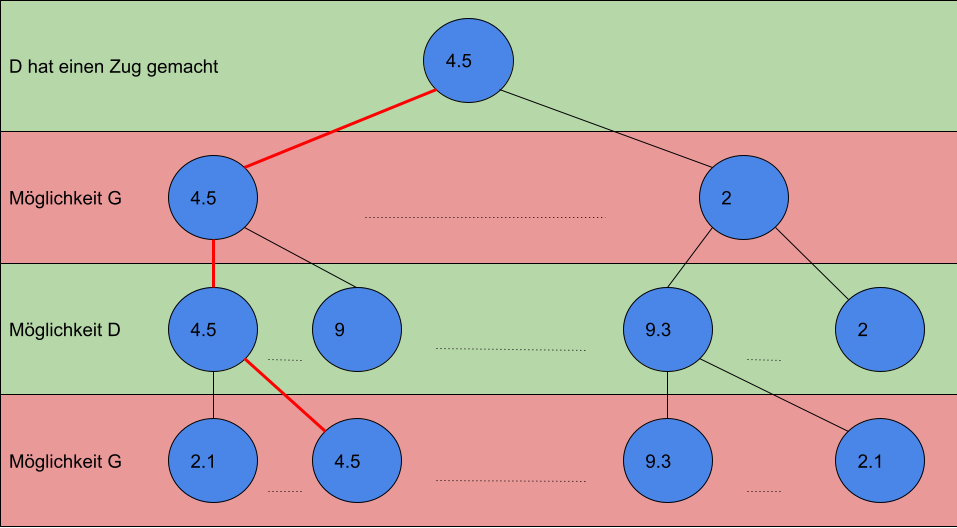
\includegraphics[width=0.5\textwidth]{../common/02_main/resources/04_gan_game_tree_filled.png}
    \end{center}
    \caption{Berechneter GAN-Game-Tree}
    \label{fig:Berechneter GAN-Game-Tree}
\end{figure}
Der rote Pfad bildet nach aktuellem Kentnisstand der beste Weg für $D$, und wird diesen wählen unter der Annahme,
dass $G$ wiederum den Weg wählen wird, welcher für $G$ am besten ist.
\newpage
\section{Lernprozess}
Der Algorithmus sieht vor, dass zuerst der Diskriminator $D$ trainiert wird. Dazu wird $k$-mal ein Minibatch aus
den Noise-Samples wie auch aus den originalen Samples geladen. Der Diskriminator wird dann anhand der Formel \ref{eq:1}
aktualisiert.
Nach diesen $k$-Schritten wird wiederum ein Minibatch von Noise-Samples geladen und der Generator damit trainiert.
Dieser Ablauf ist aus dem Algorithmus \ref{alg:1} ersichtlich, welcher von den Autoren des Papers beschrieben wird \cite{8253599}.

\begin{algorithm}[H] \label{alg:1}
    \For{number of epochs}{
        \For{k steps}{
            Sample minibatch of $m$ noise samples $\{z^{(1)}, \cdots, z^{(m)}\}$ from noise prior $p_{g}(z)$\\
            Sample minibatch of $m$ originals ${x^{(1)}, \cdots, x^{(m)}}$ from original data set $p_{data}(x)$\\
            Update the discriminator by ascending its stochastic gradient:\\
            $\nabla_{\theta_d} \frac{1}{m}\sum_{i=1}^{m}[\log D(x^{(i)}) + \log(1 - D(G(z^{(i)})))]$
        }
        Sample minibatch of $m$ noise samples $\{z^{(1)}, \cdots, z^{(m)}\}$ from noise prior $p_{g}(z)$\\
        Update the generator by descending its stochastic gradient:\\
        $\nabla_{\theta_g} \frac{1}{m}\sum_{i=1}^{m}[\log(1 - D(G(z^{(i)})))]$
    }
\end{algorithm}

\section{Noise zu Sample}
Die Problematik der Bildgenerierung an sich wurde zu Beginn ein wenig angedeutet. Dies soll nun vertieft
werden. Nach \glqq Computerphile \grqq{} lernt ein Neuronales Netz die Klassifikation auf ein Label. Das heisst, es gibt
jeweils genau eine richtige Lösung \cite[~t 4:00]{youtube:gan}. Die Problematik besteht nun darin, dass es in diesem Fall eine
unendliche Menge an korrekten Lösungen gibt. Es kann also eine Lösung bei einem \Gls{KNN} angefragt werden, die erhaltene
Lösung muss dann aber mit einer Art \glqq Zufälligkeit\grqq{} verändert, respektive korrigiert werden.
\para
Wie Eingangs erwähnt, bildet $G$ ein Mapper von Noise-Samples $z$ nach Samples in $x \in p_{data}$. Weiterhin ist nach
dem Beispiel in Tensorflow das neuronale Netz von $G$ als \Gls{CNN} definiert. Wahrscheinlich entspricht die Input-Dimension des
Bilds der Output-Dimension \cite{tensorflow:1:gan}. Damit ist die Antwort auf die Frage bereits vornweg genommen.
Die Frage selbst lautet, wie der Generator Bilder erzeugt. Um dies trotzdem ein wenig genauer zu erläutern wird zu Beginn
ein neuronales Netz angenommen, das lediglich ein einzelnes Neuron in der Input-Schicht hat. Der Definitionsbereich dieses Neurons sei
weiterhin auf $0$ und $1$ beschränkt, ist also binär. Dementsprechend kann der Generator logischerweise genau zwei Bilder
generieren, da es sich um einen deterministischen Algorithmus handelt, welcher keinerlei Zufälligkeit zulässt.
\para
Irgendwoher muss diese Zufälligkeit dem Generator zugeführt werden. Dies geschieht nun eben bei diesem Input-Layer.
Bei einem klassischen \Gls{KNN} kann es also nicht einfach nur ein Neuron geben. Es gibt eine ganze Menge und der Wert
der einzelnen Inputs kann zwischen bestimmten Intervallen liegen. Weiterhin werden alle Werte zufällig bestimmt,
was einem Rauschen gleichkommt, wie in Abbildung \ref{fig:Input-Noise} ersichtlich ist.
\begin{figure}[h!]
    \begin{center}
        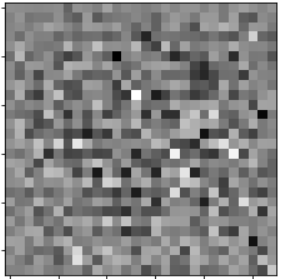
\includegraphics[width=0.5\textwidth]{../common/02_main/resources/05_noise.png}
    \end{center}
    \caption{Input-Noise \cite{tensorflow:1:gan}}
    \label{fig:Input-Noise}
\end{figure}
\para
Was genau bedeutet nun dieses Rauschen? Nach \glqq Computerphile\grqq{} kann dieses Rauschen einem Punkt in einem
mehrdimensionalen Raum gleichgesetzt werden \cite[~t 16:45]{youtube:gan}. Wird dieser Punkt leicht angepasst, dann
wird der Generator daraus ein leicht anderes Sample erzeugen, das einem Sample aus dem Datenset $p_{data}$ entspricht.
Eine Richtung in diesem mehrdimensionalen Raum kann ebenfalls bestimmten Eigenschaften zugewiesen werden. Wird der Punkt
z.B. in nur eine Richtung verschoben, so wird ein Objekt auf dem Output-Sample leicht grösser. Eine
Richtung in diesem Raum würde also der Grösse entsprechen \cite[~t 17:35]{youtube:gan}.

\section{Vor- und Nachteile}
Ein grosser Nachteil ist, dass $D$ und $G$ während dem Training synchronisiert werden müssen, $G$ kann also nicht
häufig trainiert werden ohne auch $D$ zu aktualisieren. Ansonsten könnte das \glqq Helvetica Szenario\grqq{} eintreten,
wo $G$ sehr viele Samples aus dem Noise-Raum $p_z$ auf dasselbe Sample im originalen Raum $p_x$ abbildet \cite{8253599}.
\para
Vorteile betreffen das Lernen an sich. So muss nur \Gls{Backpropagation} eingesetzt werden, um Gradienten zu finden.
Es kann auch gut sein, dass statistische Vorteile erzielt werden durch die Tatsache, dass der Generator $G$ nicht direkt
mit Samples aus den Testdaten sondern nur mit Informationen von $D$ aktualisiert wird. Die Autoren verweisen hier auf
den Fakt, dass Komponenten der Testdaten nicht direkt die Parameter des Generators beeinflussen \cite{8253599}.